
\subsection{Taxonomie}\label{taxonomie}

Taxonomie wordt gebruikt voor lijsten van woorden. Bijvoorbeeld: de lijst �FAQ categorie�n� bevat de woorden 'Netwerk' en 'Werkplekken'. Taxonomie lijsten kunnen altijd aangepast worden.

\subsubsection{Woordenlijsten toevoegen}

Om nieuwe woordenlijsten toe te voegen ga je naar: \emph{Structuur} $\rightarrow$ \emph{Taxonomie} $\rightarrow$ \emph{Woordenlijst toevoegen}, of ga direct naar \drupalpath{admin/structure/taxonomy/add}.

Vul een naam in bij het veld 'Naam' en geef eventueel een beschrijving op bij het veld 'Beschrijving'.
Klik op de knop 'Opslaan' om de woorden lijst toe te voegen.

Om woorden toe te voegen aan een lijst klik je in de meest rechter kolom op 'Termen toevoegen' bij de betreffende lijst.
Vul bij het veld 'Naam' het woord in dat je aan het lijstje wilt toevoegen, bijvoorbeeld 'Netwerk'. 
Klik onderaan de pagina op de knop 'Opslaan' om het woord toe te voegen aan de lijst. 
Herhaal deze stap om meerdere woorden toe te voegen.

\bigskip

\begin{center}
	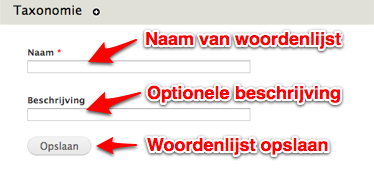
\includegraphics[width=\textwidth]{img/taxonomie1.png}
\end{center}


\subsubsection{Woordenlijsten bewerken}

Om de naam en/of beschrijving van de woordenlijst te bewerken klik je op 'Woordenlijst bewerken' bij de betreffende lijst.
Na het wijzigen klik je op de knop 'Opslaan' om de wijzigingen op te slaan.

Het is ook mogelijk om specifieke woorden uit lijsten te bewerken. Klik op 'Termen weergeven' bij de betreffende lijst.
Klik op 'Bewerken' bij het betreffende woord, vervolgens kun je de wijzigingen doorvoeren. Klik op de knop 'Opslaan' om de wijzigingen op te slaan.

\bigskip

\begin{center}
	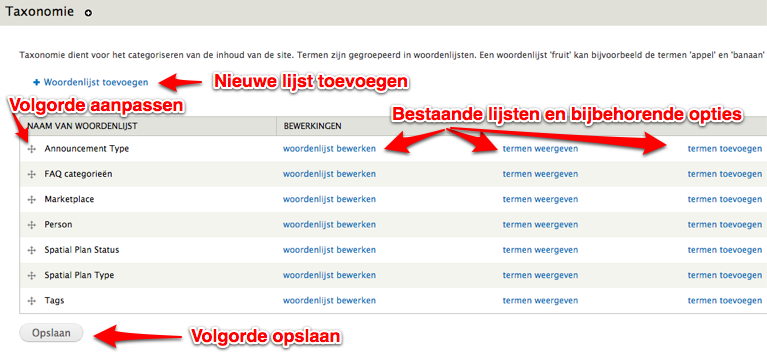
\includegraphics[width=\textwidth]{img/taxonomie2.png}
\end{center}

\subsubsection{Woordenlijsten verwijderen}

Een woordenlijst kan in ��n keer verwijderd worden, klik op 'Woordenlijst bewerken' bij de betreffende lijst en klik vervolgens op de knop 'Verwijderen'. Na het bevestigen zal de lijst definitief en onherstelbaar verwijderd worden.

Het is ook mogelijk om specifieke woorden uit lijsten te verwijderen. Klik op 'Termen weergeven' bij de betreffende lijst.
Klik op 'Bewerken' bij het betreffende woord, om het woord te verwijderen klik je onderaan de op de knop 'Verwijderen'. Na het bevestigen zal het woord definitief en onherstelbaar verwijderd worden.
